%% Lee
%% In dissertation, change 
%    section* to chapter 
%    subsection* to section
%    subsubsection* to subsection

% #######################################################################################################################################
% >>>>>>>>>>>>>>>>>>>>>>>>>>> Results <<<<<<<<<<<<<<<<<<<<<<
\chapter{Results}
\label{sec:Results}
The objectives of this work was to design a system able to accelerate multiple disparate \acp{ann} in embedded systems.
\iffalse
This means systems that are not designed to process multiple requests of essentially the same operation.
\fi
Given that these systems cannot effectively utilize \ac{sram}, the main objective was to demonstrate a system that can operate efficiently using \ac{3ddram}.
\iffalse
The system decodes instructions, sends configuration to various functions, pre-fetchs and pipelines data.
This parallelism allows the system to constantly stream data whilst results from previous operations are being operated on.
\fi

To demonstrate such a system, this work targeted \ac{3dic} technology including \ac{3ddram}. This work proposes that if a system can be purely in \ac{3dic}, the system can take advantage of the benefits
of \ac{3dic} which includes reduced energy, area and high bandwidth.
In addition, this work proposes that given the system is \ac{3dic}, then a customized \ac{dram} would provide a significant bandwidth boost over typical implementations using standard DRAM.
\iffalse
To ensure the system was purely \ac{3dic}, the area of the system Manager and Processing Engine has to stay within the physical footprint of the \ac{3ddram}.
\fi

Therefore, the objective of this work is to demonstrate the proposed system can maintain the required data bandwidth all whilst staying within the physical footprint of the \ac{3ddram}. 


The target technology node was \SI{28}{\nano\meter}, mainly because its the technology node employed for some recent \acp{gpu} and other \acp{asic} such as \cite{jouppi2017datacenter}.
A full \SI{28}{\nano\meter} technology node was not available to this team because the logic library did not have compiler support for register files.
Therefore, the design was synthesized using an available \SI{65}{\nano\meter} technology node, which does have \ac{sram} and register file compiler support and then scaled to \SI{28}{\nano\meter}.
%There are techonlogy scaling number available \cite{schabel2017energy}, but the scaling numbers used by this work were generated by synthesizing a representative design from this work which did not employ register files.
%The module chosen was the \ac{dram} memory controller.

\section{Power and Area Scaling estimates}
\label{sec:Power and Area Scaling estimates}

To obtain scaling numbers, portions of the design were synthesized using the \SI{28}{\nano\meter} library.
The area and power results from these synthesis runs are shown in table was used to generate the power and area scaling numbers shown in table \ref{tab:Scaling runs}.
The final scaling numbers are shown in table \ref{tab:Scaling}.

\begin{table}[h]
  % the [] contains position info e.g. [!t] means here
  \centering
  \captionsetup{justification=centering}

  \begin{minipage}{1\textwidth}
    \centering
    \begin{minipage}{0.65\textwidth}
        \begin{adjustbox}{width=1\textwidth}
            \footnotesize
            \begin{tabular}{ |c|c|c|c|c|c|  }
              \hline
              %\rowcolor{gray!50}
              %\multicolumn{5}{|c|}{Power } \\
              %\hline
              %\rowcolor{gray!25}
          Node  &   Type & Frequency                              & Internal                & Net switching           & Leakage                  \\
              \hline
          \SI{65}{\nano\meter}  &  Logic &\SI[per-mode=symbol]{100}{\mega\hertz}  & \SI{66.9}{\milli\watt} & \SI{1.53}{\milli\watt} & \SI{2.02}{\nano\watt}  \\  % xls
          \SI{28}{\nano\meter}  &  Logic &\SI[per-mode=symbol]{100}{\mega\hertz}  & \SI{13.2}{\milli\watt} & \SI{1.26}{\milli\watt} & \SI{4.9 }{\micro\watt} \\  % xls
          %\SI{65}{\nano\meter}  &  Logic &\SI[per-mode=symbol]{100}{\mega\hertz}  & \SI{142}{\milli\watt} & \SI{123}{\milli\watt} & \SI{192}{\micro\watt}  \\  % main_mem_cntl
          %\SI{28}{\nano\meter}  &  Logic &\SI[per-mode=symbol]{100}{\mega\hertz}  & \SI{ 28}{\milli\watt} & \SI{100}{\milli\watt} & \SI{22.4}{\milli\watt} \\  % main_mem_cntl
%      Scaling  &                                                 & \num{5.06}              & \num{1.22}              & \num{4.11e-3}            \\
              \hline
            \end{tabular}
        \end{adjustbox}
      \subcaption{Example logic only design synthesis power}
      \label{tab:Scaling}
    \end{minipage}
    \begin{minipage}{0.65\textwidth}
        \vspace{5mm}
        \begin{adjustbox}{width=1\textwidth}
            \footnotesize
            \begin{tabular}{ |c|c|c|c|c|c|  }
              \hline
              %\rowcolor{gray!50}
              %\multicolumn{5}{|c|}{Power } \\
              %\hline
              %\rowcolor{gray!25}
          Node  & Type      & Frequency                              & Internal                & Net switching           & Leakage                 \\
              \hline
          \SI{65}{\nano\meter}  & Memory    & \SI[per-mode=symbol]{100}{\mega\hertz}  & \SI{2.36}{\milli\watt}  & \SI{0.6}{\micro\watt}  & \SI{5.4}{\pico\watt}    \\   % wu_memory
%          \SI{65}{\nano\meter} & Register  & \SI[per-mode=symbol]{100}{\mega\hertz}  & \SI{61  }{\micro\watt}  & \SI{6  }{\micro\watt}  & \SI{12.6}{\nano\watt}   \\
%          \SI{65}{\nano\meter} & Comb      & \SI[per-mode=symbol]{100}{\mega\hertz}  & \SI{  }{\micro\watt}    & \SI{6  }{\micro\watt}  & \SI{12.6}{\nano\watt}   \\
          \SI{28}{\nano\meter}  & Memory    & \SI[per-mode=symbol]{100}{\mega\hertz}  & \SI{43.8}{\micro\watt}  & NR                     & \SI{443}{\micro\watt}   \\   % wu_memory
%          \SI{28}{\nano\meter} & Logic     & \SI[per-mode=symbol]{100}{\mega\hertz}  & \SI{2.8 }{\micro\watt}  & \SI{0.38}{\micro\watt} & \SI{0.53}{\micro\watt}  \\
%       Scaling &                                                     & \num{5.06}              & \num{1.22}             & \num{4.11e-3}           \\
              \hline
            \end{tabular}
        \end{adjustbox}
      \subcaption{Example design with memory synthesis power}
      \label{tab:Example design with memory synthesis power}
    \end{minipage}
    \begin{minipage}{0.65\textwidth}
        \vspace{5mm}
        \begin{adjustbox}{width=1\textwidth}
            \footnotesize
            \begin{tabular}{ |c|c|c|c|  }
              \hline
              %\rowcolor{gray!50}
              %\multicolumn{5}{|c|}{Power } \\
              %\hline
              %\rowcolor{gray!25}    % wu_memory                                        1024x50                               
          Node  & Type      & Area from synthesis                                 & Area from Datasheet                                \\
              \hline
          \SI{65}{\nano\meter}  & Logic     & \SI[per-mode=symbol]{879593}{\square\micro\meter}  & NA\\ %\SI[per-mode=symbol]{57014}{\square\micro\meter}    \\
          \SI{28}{\nano\meter}  & Logic     & \SI[per-mode=symbol]{327822}{\square\micro\meter}  & NA\\ %\SI[per-mode=symbol]{20281}{\square\micro\meter}    \\
          \SI{65}{\nano\meter}  & Memory    & \SI[per-mode=symbol]{210230}{\square\micro\meter}  & \SI[per-mode=symbol]{57014}{\square\micro\meter}    \\
          \SI{28}{\nano\meter}  & Memory    & \SI[per-mode=symbol]{75605 }{\square\micro\meter}  & \SI[per-mode=symbol]{20281}{\square\micro\meter}    \\
%      Scaling  &           & \num{5.06}                                         & \num{1.22}                                          \\
              \hline
            \end{tabular}
        \end{adjustbox}
      \subcaption{Example design area}
      \label{tab:Example design area}
    \end{minipage}
  \end{minipage}
  \captionsetup{justification=centering, skip=9pt}
  \vspace{0.0cm}
  \captionof{table}{Example design area and power}
  \label{tab:Scaling runs}
\end{table}

\begin{table}[h]
  % the [] contains position info e.g. [!t] means here
  \centering
  \captionsetup{justification=centering}
  \begin{minipage}{1\textwidth}
    \centering
    \begin{minipage}{0.85\textwidth}
        \vspace{5mm}
        \begin{adjustbox}{width=1\textwidth}
            \footnotesize
            \begin{tabular}{|>{\centering}m{1cm}|>{\centering}m{1cm}|>{\centering}m{1cm}|>{\centering}m{1.3cm}|>{\centering}m{1.3cm}|>{\centering}m{1cm}|>{\centering}m{1.3cm}|m{1.3cm}|}\cline{3-8}
              %\hline
              %\rowcolor{gray!50}
              %\multicolumn{5}{|c|}{Power } \\
              %\hline
              %\rowcolor{gray!25}  
         \multicolumn{2}{c|}{}                                          & \multicolumn{3}{c|}{Logic power}                                                                  &  \multicolumn{3}{c|}{Memory power}                                                                                                                                  \\\cline{1-8}
         Logic Area                  & Memory Area                      & Internal                            & Net switching                  & Leakage                    & Internal                                                                                                              & Net switching                  & Leakage    \\\cline{1-8}
          \num{2.68}                 & \num{2.78}                       &  \num{5.07}                         & \num{1.21}                     & \num{4.12e-4}              & \num{5.07}\footnote{this number is conservative based on table \ref{tab:Example design with memory synthesis power}}  & NA                             & NA         \\
              \hline
            \end{tabular}
        \end{adjustbox}
      %\subcaption{Example design area}
      %\label{tab:Example design area}
    \end{minipage}
  \end{minipage}
  \captionsetup{justification=centering, skip=9pt}
  \vspace{0.0cm}
  \captionof{table}{\SI{68}{\nano\meter} to \SI{28}{\nano\meter} scaling numbers}
  \label{tab:Scaling numbers}
\end{table}

\section{Physical Placement}
\label{sec:Physical Placement}

Based on the \ac{diram4} layout shown in in figure \ref{fig:diram4Layout}, the dimensions of the area available for each \ac{ssc} is \SI{1470}{\micro\meter} by \SI{1656}{\micro\meter} or approximately \SI{2.43}{\square\milli\meter}.
Using the logic and memory scaling numbers from table \ref{tab:Scaling numbers}, the effective dimensions at \SI{65}{\nano\meter} is \SI{2431}{\micro\meter} by \SI{2738}{\micro\meter} providing a design area at \SI{65}{\nano\meter} of approximately \SI{6.66}{\square\milli\meter}.

The area contribution of each block within the Manager and \ac{pe} can be seen in table \ref{tab:Area contribution}.
\begin{table}[h]
%  \captionsetup{justification=centering, skip=-5pt}
  \captionsetup{justification=centering, skip=3pt}
  \caption{Area contribution}
  \vspace{3pt}
  \label{tab:Area contribution}
  \centering
    % [lr] ~ left align col 0 and right align col 1
    % e.g. 4 columns could be lccr
  \begin{subtable}{1\textwidth}
    \centering
    \begin{adjustbox}{width=0.50\textwidth}
      \begin{tabular}{|c|c|c|}
        \hline
                            % \multicolumn{4}{c}{3D-DRAM Simulation-based estimates}   \\
       \multirow{2}{*}{Block name}    &  \multirow{2}{*}{Instances}        &  \multirow{2}{*}{Percentage contribution}     \\  %\cline{1-1}
                                      &                                    &                                               \\
        \hline  % instead of \midrule %midrule doesnt overlap with column lines
  Memory Controller      & 1&\SI[per-mode=symbol]{20.5}{\percent}  \\ 
        NoC              & 1&\SI[per-mode=symbol]{ 6.9}{\percent}  \\
        Read Control     & 2&\SI[per-mode=symbol]{46.8}{\percent}  \\
        Write Control    & 1&\SI[per-mode=symbol]{ 7.2}{\percent}  \\
      Instruction Proc   & 1&\SI[per-mode=symbol]{ 1.7}{\percent}  \\
      Return Data Proc   & 1&\SI[per-mode=symbol]{ 1.6}{\percent}  \\
      System Controller  & 1&\SI[per-mode=symbol]{ 1.6}{\percent}  \\
        TSV              &NA&\SI[per-mode=symbol]{ 6.9}{\percent}  \\
        Misc             &NA&\SI[per-mode=symbol]{}{\percent}  \\
        \hline
      \end{tabular}
    \end{adjustbox}
    \vspace{3pt}
    \captionsetup{justification=centering, skip=10pt}
    \caption{Manager}
    \label{tab:Manager Area Contribution}
  \end{subtable}
  \bigskip
  \begin{subtable}{1\textwidth}
    \centering
    \begin{adjustbox}{width=0.55\textwidth}
      \begin{tabular}{|c|c|c|}
        \hline
                            % \multicolumn{4}{c}{3D-DRAM Simulation-based estimates}   \\
       \multirow{2}{*}{Block name}    &  \multirow{2}{*}{Instances}        &  \multirow{2}{*}{Percentage contribution}     \\  %\cline{1-1}
                                      &                                    &                                               \\
        \hline  % instead of \midrule %midrule doesnt overlap with column lines
     Operation Decode    & 1&\SI[per-mode=symbol]{ 3.3}{\percent}  \\
   Return Data Control   & 1&\SI[per-mode=symbol]{ 1.5}{\percent}  \\
    SIMD Wrapper         & 1&\SI[per-mode=symbol]{11.2}{\percent}  \\
        SIMD             & 1&\SI[per-mode=symbol]{18.7}{\percent}  \\
  Streaming Operations   &32&\SI[per-mode=symbol]{41.8}{\percent}  \\
  Streaming Op Control   & 1&\SI[per-mode=symbol]{ 2.0}{\percent}  \\
 Local Memory + Control\footnote{A small amount of scratchpad memory was provided between \acp{stop} and \ac{simd} but in practice could be much smaller. It is not used in any of the fanin tests.}  & 1&\SI[per-mode=symbol]{17.7}{\percent}  \\ 
        TSV              &NA&\SI[per-mode=symbol]{ 3.9}{\percent}  \\
        Misc             &NA&\SI[per-mode=symbol]{ 0.5}{\percent}  \\
        \hline
      \end{tabular}
    \end{adjustbox}
    \vspace{3pt}
    \captionsetup{justification=centering, skip=10pt}
    \caption{PE}
    \label{tab:PE Area Contribution}
  \end{subtable}
  \end{table}

The layout utilization for the manager and \ac{pe} are \SI{81.5}{\percent} and \SI{50}{\percent} respectively.
The utilization suggests the manager is clearly more challenging to place and route.
To get a sense of the physical feasibility of the system, both the manager and \ac{pe} were placed and routed without \ac{drc} using Synopsys\textregistered ~IC Compiler\texttrademark.
A route congestion analysis was performed which indicated very few congested areas, which was most likely due to the wide datapath nature of the design.
A preliminary place and route for the Manager and \ac{pe} are shown in figure \ref{fig:Manager and PE Die layouts}. 
The physical placement and congestion of the manager and \ac{pe} suggests a relatively low risk of completing a full detailed place and route.

\begin{figure}[h]
\centering
\begin{subfigure}{.5\textwidth}
  \centering
  \centerline{
    \mbox{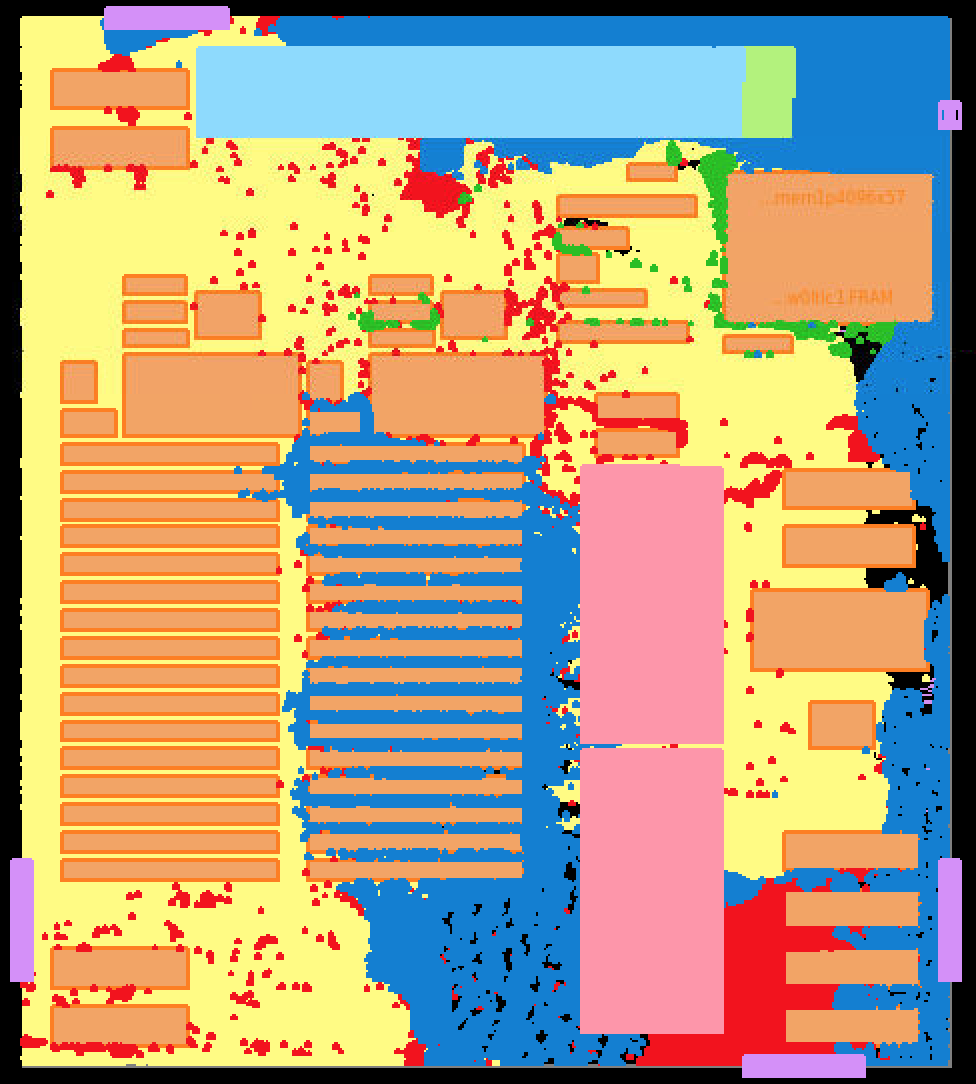
\includegraphics[width=1\linewidth]{ManagerLayout.png}}
  }
  \captionsetup{justification=centering, width=.8\linewidth}
  \caption{Manager}
  %\vspace{40pt}
  \label{fig:managerLayout}
\end{subfigure}%

\bigskip

\begin{subfigure}{.5\textwidth}
  \centering
  \centerline{
    \mbox{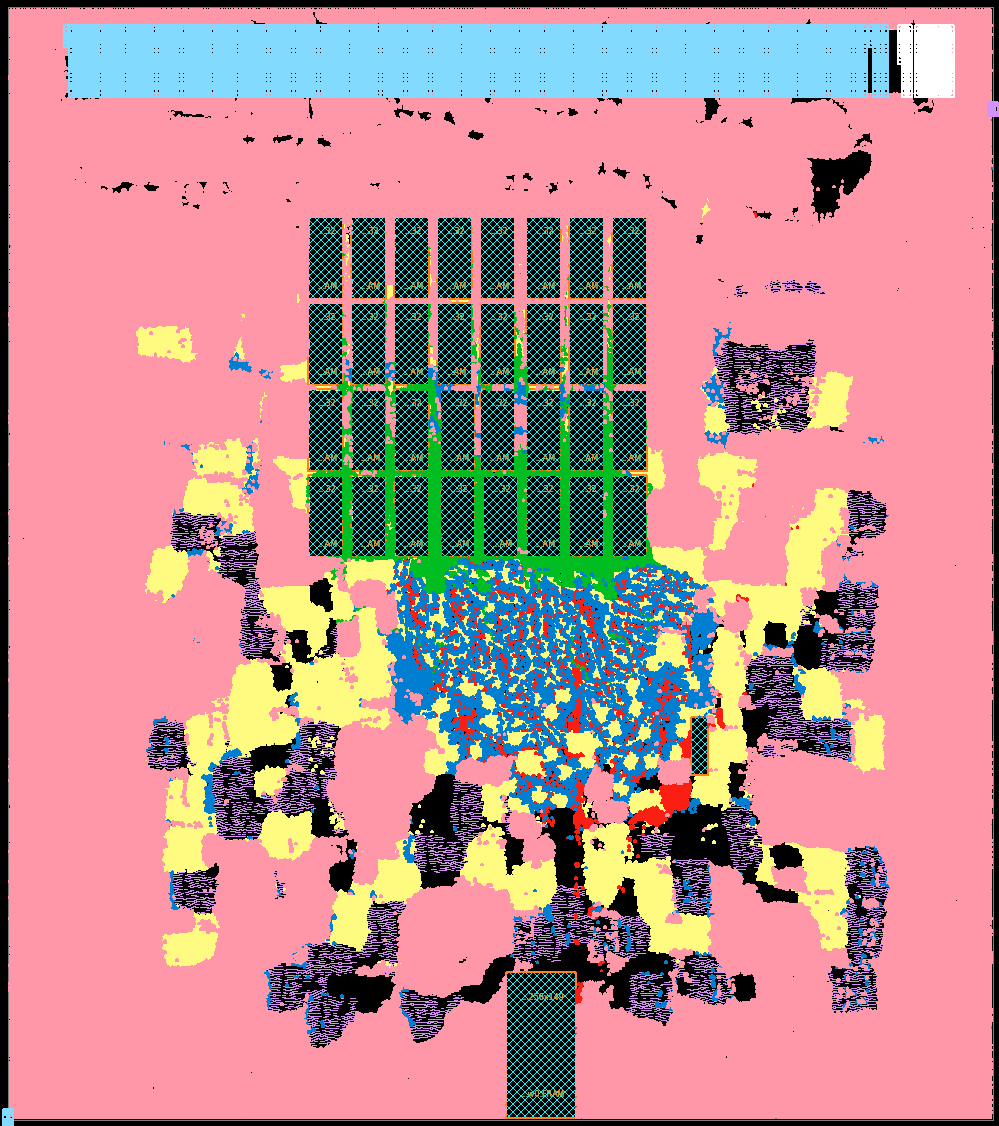
\includegraphics[width=1\linewidth]{PElayout.png}}
  }
  \captionsetup{justification=centering, width=.8\linewidth}
  \caption{PE}
  \label{fig:peLayout}
\end{subfigure}
\captionsetup{justification=centering, width=.9\linewidth}
\caption{Manager and PE Die layouts}
\label{fig:Manager and PE Die layouts}
\end{figure}



\section{Synthesis}
\label{sec:Synthesis}

%The design has been coded . 
To determine the appropriate frequency scaling between \SI{28}{\nano\meter} and \SI{65}{\nano\meter}, an example logic-only design was synthesized using the \SI{28}{\nano\meter} and \SI{65}{\nano\meter} libraries. 
In each case, the frequency was increased until negative timing slack was observed.
This suggested that to achieve an operating frequency of \SI{500}{\mega\hertz} at \SI{28}{\nano\meter} the design should be synthesized at \SI{65}{\nano\meter} using a frequency of \SI{193}{\mega\hertz}.
All blocks in the system were synthesized using a typical library and no blocks had issues synthesizing using the typical library at this relatively low frequency suggesting a target frequency of \SI{500}{\mega\hertz} at \SI{28}{\nano\meter} is relatively low risk.


\iffalse
As mention previously \eqref{eq:averageBandwidth}, to process multiple useful sized \acp{ann} requires a sustained bandwidth to the \ac{pe} of the order of ten's of \SI[per-mode=symbol]{}{\tera\bit\per\second}.
\fi

%%%%The approximate design targets are shown in Table \ref{tab:DesignTargets}.
%%%%
%%%%\begin{table}[h]
%%%%%  \captionsetup{justification=centering, skip=-5pt}
%%%%  \captionsetup{justification=centering, skip=3pt}
%%%%  \caption{Design targets}
%%%%  \label{tab:DesignTargets}
%%%%  \centering
%%%%%  \begin{center}
%%%%    % [lr] ~ left align col 0 and right align col 1
%%%%    % e.g. 4 columns could be lccr
%%%%    \begin{tabular}{lr}
%%%%      \toprule
%%%%      Parameter         & Target \\
%%%%      \midrule
%%%%      Frequency         & $>$\SI{700}{\MHz}   \\
%%%%      Power             & \SI{\approx 80}{\W}   \\
%%%%      Bandwidth         & \SI[per-mode=symbol]{\approx 64}{\tera\bit\per\second} \\
%%%%      Overall Die Area  & \SI{175}{\mm^2} \\
%%%%      \bottomrule
%%%%    \end{tabular}
%%%%%  \end{center}
%%%%\end{table}


\section{Logic Verification}
\label{sec:Logic Verification}

The primary control and datapaths of the system have been simulated in a system verilog environment using Mentor Graphics\textregistered ~ModelSim\texttrademark.
To ensure a high bandwidth utilization can be maintained, a group of tests representing convolutional and fully connected layers were simulated.
The operations simulated were based on the expected lower and upper limits of pre-synaptic fanin. 
These testcases were based on layers similar to CONV2 and FC-7 from \cite{krizhevsky2012imagenet} which represent a pre-synaptic fanin of 225 and 4000 respectively.
Additional testcases were employed representing pre-synaptic fanins of 294, 300, 500 and 1000. Both locally connected (CONV) and fully connected (FC) type fanins were tested.
To understand the test notation, the tests labelled CONV-500 and FC-500 represent convolutional and fully-connected tests respectively both with a pre-synaptic fanin of 500.
The results showing sustained average bandwidth can be seen in table \ref{tab:Bandwidth Estimates}.


\begin{table}[h]
%  \captionsetup{justification=centering, skip=-5pt}
  \captionsetup{justification=centering, skip=3pt}
  \caption{Fanin bandwidth tests}
  \vspace{3pt}
  \label{tab:Bandwidth Estimates}
  \centering
    \begin{adjustbox}{width=0.45\textwidth}
      \begin{tabular}{|c|c|c|}
        %\toprule
        \hline
                            % \multicolumn{4}{c}{3D-DRAM Simulation-based estimates}   \\
               \multirow{3}{*}{Test}                   &                                         \multicolumn{2}{c|}{\multirow{2}{*}{Average Bandwidth at frequency}}  \\
                                                       &                                         \multicolumn{2}{c|}{}                                                 \\ \cline{2-3} % still need line even though cells are defined
                                                       &        \SI{500}{\mega\hertz}                            & \SI{700}{\mega\hertz}                               \\%  \cline{1-3}
        \hline  % instead of \midrule %midrule doesnt ove        
                   CONV2 \cite{krizhevsky2012imagenet} &\ \SI[per-mode=symbol]{\sim 22}{\tera\bit\per\second}    & \SI[per-mode=symbol]{\sim 30}{\tera\bit\per\second} \\ %\cline{2-2}
                   CONV-294                            &\ \SI[per-mode=symbol]{\sim 23}{\tera\bit\per\second}    & \SI[per-mode=symbol]{\sim 31}{\tera\bit\per\second} \\ %\cline{2-2}
                   CONV-300                            &\ \SI[per-mode=symbol]{\sim 25}{\tera\bit\per\second}    & \SI[per-mode=symbol]{\sim 34}{\tera\bit\per\second} \\ %\cline{2-2}
                   CONV-500                            &\ \SI[per-mode=symbol]{\sim 26}{\tera\bit\per\second}    & \SI[per-mode=symbol]{\sim 38}{\tera\bit\per\second} \\ %\cline{2-2}
                   CONV-1000                           &\ \SI[per-mode=symbol]{\sim 30}{\tera\bit\per\second}    & \SI[per-mode=symbol]{\sim 41}{\tera\bit\per\second} \\ %\cline{2-2}
                   FC-350                              &\ \SI[per-mode=symbol]{\sim 26}{\tera\bit\per\second}    & \SI[per-mode=symbol]{\sim 36}{\tera\bit\per\second} \\ %\cline{2-2}
                   FC-500                              &\ \SI[per-mode=symbol]{\sim 27}{\tera\bit\per\second}    & \SI[per-mode=symbol]{\sim 38}{\tera\bit\per\second} \\ %\cline{2-2}
                   FC-1000                             &\ \SI[per-mode=symbol]{\sim 30}{\tera\bit\per\second}    & \SI[per-mode=symbol]{\sim 42}{\tera\bit\per\second} \\ %\cline{2-2}
                   FC-7 \cite{krizhevsky2012imagenet}  &\ \SI[per-mode=symbol]{\sim 31}{\tera\bit\per\second}    & \SI[per-mode=symbol]{\sim 43}{\tera\bit\per\second} \\ %\cline{2-2}
        \hline
        %\bottomrule
      \end{tabular}
    \end{adjustbox}
    \vspace{3pt}
  \end{table}


\section{Power Estimates}
\label{sec:Power Estimates}

To estimate power consumption, the parasitics were extracted from the preliminary layouts and simulated against a representative testcase.
The power testcase employed was the CONV2.
The simulation generated an activity file which was then used by the Synopsys\textregistered ~Primetime-PX\texttrademark ~power analysis tool to obtain power and bandwidth estimates.
The \ac{dram} accesses were captured and \ac{dram} power dissipation calculated from \cite{tezzaron:diram4}. The power dissipated in the TSVs were estimated from \cite{liu2012compact}.
These estimates were scaled using the scaling numbers from table \ref{tab:Scaling runs} and used to estimate power dissipation for operating frequencies of \SI{500}{\mega\hertz} and \SI{700}{\mega\hertz} using a \SI{28}{\nano\meter} techology node.
The estimated overall power along with per block contribution are shown in table \ref{tab:Simulation-based estimates}.

\begin{table}[h]
%  \captionsetup{justification=centering, skip=-5pt}
  \captionsetup{justification=centering, skip=3pt}
  \caption{Power Estimates}
  \vspace{3pt}
  \label{tab:Simulation-based estimates}
  \centering
    % [lr] ~ left align col 0 and right align col 1
    % e.g. 4 columns could be lccr
  \begin{subtable}{1\textwidth}
    \centering
    \begin{adjustbox}{width=0.70\textwidth}
      \begin{tabular}{|c|c|c|c|}
       \hline
       \multirow{2}{*}{Technology node}    &  \multirow{2}{*}{Clock frequency}        &  \multirow{2}{*}{Total expected power}   &  \multirow{2}{*}{Testcase}     \\  %\cline{1-1}
                                           &                                          &                                          &                                \\\hline
       \SI{28}{\nano\meter}                & \SI{500}{\mega\hertz}                    &   \SI{72.5}{\watt}                       &  CONV-294\iffalse \SI[per-mode=symbol]{\sim 70}{\percent} \fi \\ %\cline{2-2}
       \SI{28}{\nano\meter}                & \SI{700}{\mega\hertz}                    &   \SI{96.5}{\watt}                       &  CONV-294\iffalse \SI[per-mode=symbol]{\sim 70}{\percent} \fi \\ %\cline{2-2}
        \hline
      \end{tabular}
    \end{adjustbox}
    \vspace{3pt}
    \captionsetup{justification=centering, skip=10pt}
    \caption{Power Dissipation}
    \label{tab:Power Dissipation}
  \end{subtable}
  \bigskip
  \begin{subtable}{0.75\textwidth}
    \centering
    \begin{adjustbox}{width=0.55\textwidth}
      \begin{tabular}{|c|c|}
        \hline
       \multirow{2}{*}{Block name}    &  \multirow{2}{*}{Percentage contribution}    \\
                                      &                                              \\\hline
                Manager  & \SI[per-mode=symbol]{58.7}{\percent}  \\ 
                     PE  & \SI[per-mode=symbol]{36.5}{\percent}  \\
                   DRAM  & \SI[per-mode=symbol]{ 2.2}{\percent}  \\
              DRAM TSVs  & \SI[per-mode=symbol]{ 1.6}{\percent}  \\
         Stack Bus TSVs  & \SI[per-mode=symbol]{ 1.0}{\percent}  \\
        \hline
      \end{tabular}
    \end{adjustbox}
    \vspace{3pt}
    \captionsetup{justification=centering, skip=10pt}
    \caption{Power Contribution}
    \label{tab:Power Dissipation}
  \end{subtable}
  \end{table}


\section{Summary}
\label{sec:Results summary}

The bandwidth performance shown in table \ref{tab:Bandwidth Estimates} shows a sustained average bandwidth that exceeds the requirement shown in table \ref{tab:Bandwidth and Storage Design Requirements}.
When using this work in a full system with data transfers between a host and the \ac{ssc}, there will be idle times but this should have a relatively low impact as it involves mostly input download and result upload.
The focus of the veriication environment was the \ac{an} processing which involves the most complex operations in the system, including memory management, flow control etc.
The \ac{bootp} process was simulated along with host memory upload and download, mainly to ensure the major datapath infrastructure was in place to ensure further features would have minimal impact on the area study.
The list of features implemented and verified are shown in table \ref{tab:Features implemented}.

\begin{table}[h]
  % the [] contains position info e.g. [!t] means here
  \centering
  \captionsetup{justification=centering}

  \begin{minipage}{1\textwidth}
    \centering
      %\begin{adjustbox}{width=0.85\textwidth}
          \footnotesize
          %\begin{tabular}{|>{\centering}m{1cm}|>{\centering}m{1cm}|>{\centering}m{1cm}|>{\centering}m{1.3cm}|>{\centering}m{1.3cm}|}\cline{1-4}
          %\begin{tabular}{ |>{\centering}m{1.5cm}|>{\centering}m{1.5cm}|>{\centering}m{1.5cm}|m{3cm}|}
          \begin{tabular}{ |m{4cm}|c|c|c|m{3cm}|}
            %\hline
            %\rowcolor{gray!50}
            %\multicolumn{5}{|c|}{Power } \\
            \hline
            %\cline{1-4}
            \rowcolor{gray!25}
 \multicolumn{1}{|c|}{Feature}          &   \multicolumn{2}{c|}{Limitations}                 & Method                  &   \multicolumn{1}{c|}{Comment}                                         \\
            \hline                                                                                                     
        Major processing datapaths      &   \multicolumn{2}{c|}{N}                           & Self checking           &  \multicolumn{1}{c|}{Instructions generated using python scripts}      \\\cline{1-5}
        SIMD Wrapper special functions  &   \multicolumn{2}{c|}{N}                           & \multirow{7}{*}{Visual} &  \multicolumn{1}{c|}{\multirow{7}{*}{Instructions manually generated}} \\\cline{1-3}
        Sync Send                       &   \multicolumn{2}{c|}{Host only}                   &                         &                                                                        \\\cline{1-3}
        Sync Wait                       &   \multicolumn{2}{c|}{Host only}                   &                         &                                                                        \\\cline{1-3}
        Memory Upload                   &   \multicolumn{2}{c|}{Host from \ac{dram}}         &                         &                                                                        \\\cline{1-3}
 \multirow{2}{*}{Memory Download}       &   Solicited   & \multirow{2}{*}{Host to \ac{dram}} &                         &                                                                        \\\cline{2-2}
                                        &   Unsolicited &                                    &                         &                                                                        \\\cline{1-3}
        BootP                           &   \multicolumn{2}{c|}{N}                           &                         &                                                                        \\\cline{1-5}
        %MAC                             &   N                     & Self checking  &  Instructions generated using python scripts \\
            %\hline
          \end{tabular}
      %\end{adjustbox}
  \end{minipage}
  \captionsetup{justification=centering, skip=9pt}
  \vspace{0.0cm}
  \captionof{table}{System features implemented}
  \label{tab:Features implemented}
\end{table}

The design has been conservatively coded to ensure there are opportunities for logic reduction. For example, in all the modules \acp{fifo} have been employed at primary interfaces and the depths of those \acp{fifo} are generous 
to avoid debugging flow control issues rather than debugging the system as a whole.
In the design of \acp{fsm}, again the number of states has been assigned conservatively.
The major interfaces between blocks are all registered but this is considered a requirement when designing a system of this size.
The area scaling numbers employed are within a reasonable range based on \cite{schabel2017energy} and perhaps a little low based on \cite{schabel2014diss}.
Therefore the place and route feasibility study suggests that embarking on productizing a system based on this work would be relatively low risk.

The power numbers were higher than expected %but the power still within a number that is still considered manageable when the design is run at \SI{500}{\mega\hertz}.
and the power per unit area of \SI[per-mode=symbol]{197}{\milli\watt\per\square\milli\meter\per\giga\hertz} appears to be a high when compared to the \SI[per-mode=symbol]{133}{\milli\watt\per\square\milli\meter\per\giga\hertz} inferred from \cite{tensorflow2015-whitepaper}.
Therefore there may either be be opportunities for power reduction, such as clock gating or a fully completed place and route may result in lower power numbers.
%There is unlikely opportunities for clock gating because most of the logic is active during the processing of an \ac{ann}.
%The power numbers seem high but there is likely room for improvement when productizing the system.



